% Copyright 2021-2022 Bas van Meerten and Wouter Franssen
%
%This file is part of magpie.
%
%magpie is free software: you can redistribute it and/or modify
%it under the terms of the GNU General Public License as published by
%the Free Software Foundation, either version 3 of the License, or
%(at your option) any later version.
%
%magpie is distributed in the hope that it will be useful,
%but WITHOUT ANY WARRANTY; without even the implied warranty of
%MERCHANTABILITY or FITNESS FOR A PARTICULAR PURPOSE.  See the
%GNU General Public License for more details.
%
%You should have received a copy of the GNU General Public License
%along with magpie. If not, see <http://www.gnu.org/licenses/>.

\documentclass[11pt,a4paper]{article}
% Copyright 2016 - 2021 Bas van Meerten and Wouter Franssen
%
%This file is part of ssNake.
%
%ssNake is free software: you can redistribute it and/or modify
%it under the terms of the GNU General Public License as published by
%the Free Software Foundation, either version 3 of the License, or
%(at your option) any later version.
%
%ssNake is distributed in the hope that it will be useful,
%but WITHOUT ANY WARRANTY; without even the implied warranty of
%MERCHANTABILITY or FITNESS FOR A PARTICULAR PURPOSE.  See the
%GNU General Public License for more details.
%
%You should have received a copy of the GNU General Public License
%along with ssNake. If not, see <http://www.gnu.org/licenses/>.

\usepackage[british]{babel}
\usepackage{graphicx,booktabs,listings,amsmath,pgfplots,pgfplotstable}
\usepackage[small,bf,nooneline]{caption}
\usepackage{subcaption}
\usepackage[sort&compress,numbers]{natbib}
\usepackage{tikz}
\usepackage{mathtools}
\usepackage[nottoc]{tocbibind}%adds bibliography to table of contents.
\graphicspath{{./images/}}
%\setlength{\textwidth}{453pt} %597 pt is the a4 paperwidth. Minus 2 in margin. 72 pt = 1 in
%\setlength{\hoffset}{-\oddsidemargin}
%\setlength{\voffset}{-30pt} %
%\setlength{\textheight}{651 pt} %a4 height 845 pt minus 2* total headheight. In this case 2*88pt
%% examine margines via the layout package. Use command \layout{} in document to draw a picture.
%\setlength{\parindent}{0.5 cm}
%\setlength{\parskip}{0 cm}
\usepackage[left=82pt,right=82pt,top=95pt,bottom=95pt,footnotesep=0.5cm]{geometry}
%\setlength{\headheight}{14pt}

%define colours--------------------
%dark
\usepackage{xcolor}
\definecolor{MyGrayD}{RGB}{1,1,1}
\definecolor{MyRedD}{RGB}{237,45,46}
\definecolor{MyGreenD}{RGB}{0,140,71}
\definecolor{MyBlueD}{RGB}{24,89,169}
\definecolor{MyOrangeD}{RGB}{243,125,34}
\definecolor{MyPurpleD}{RGB}{102,44,145}
\definecolor{MyBrownD}{RGB}{161,29,32}
\definecolor{MyPinkD}{RGB}{179,56,147}
%normal
\definecolor{MyGray}{RGB}{114,114,114}
\definecolor{MyRed}{RGB}{241,89,95}
\definecolor{MyGreen}{RGB}{121,195,106}
\definecolor{MyBlue}{RGB}{89,154,211}
\definecolor{MyOrange}{RGB}{249,166,90}
\definecolor{MyPurple}{RGB}{158,102,171}
\definecolor{MyBrown}{RGB}{205,112,88}
\definecolor{MyPink}{RGB}{215,127,179}
%light
\definecolor{MyGrayL}{RGB}{204,204,204}
\definecolor{MyRedL}{RGB}{242,174,172}
\definecolor{MyGreenL}{RGB}{216,228,170}
\definecolor{MyBlueL}{RGB}{184,210,235}
\definecolor{MyOrangeL}{RGB}{242,209,176}
\definecolor{MyPurpleL}{RGB}{212,178,211}
\definecolor{MyBrownL}{RGB}{221,184,169}
\definecolor{MyPinkL}{RGB}{235,191,217}
%----------------------------------

%Figure ref with hyperref
\newcommand{\fref}[1]{\hyperref[#1]{Figure \ref*{#1}}}
\newcommand{\sref}[1]{\hyperref[#1]{Section \ref*{#1}}}
\newcommand{\tref}[1]{\hyperref[#1]{Table \ref*{#1}}}

%Makes a new command for figures with input values: filename, width(times linewidth),
% caption and label.
\newcommand{\onefigure}[4]{
\setlength{\captionwidth}{#2\linewidth}
\begin{figure}
\includegraphics[width=#2\linewidth]{#1}
\centering
\parbox{\linewidth}{\caption{#3}
\label{#4}}
\end{figure}
}

%Makes a new command for tikz figures with input values: tikz commands, 
% caption and label.
\newcommand{\onetikz}[3]{
\settowidth{\captionwidth}{#1}
\ifthenelse{\lengthtest{\captionwidth<0.7\linewidth}}{\setlength{\captionwidth}{0.7\linewidth}}{}

\begin{figure}
\centering
#1
\centering
\parbox{\linewidth}{\caption{#2}
\label{#3}}
\end{figure}
}

%Makes a new command for two figures next to each other with input values: filename1, caption1, label1,filename2, caption2 and label2. Figure width is set to 0.47\linewidth and the space between the figures is filled with \hfill so the sides of the figures align with to edge of the line.
\newcommand{\twofigure}[6]{
\setlength{\captionwidth}{\linewidth}
\begin{figure*}[ht!]
\begin{minipage}[t]{0.47\linewidth}
\includegraphics[width=\linewidth]{#1}
\centering
\caption{#2}
\label{#3}
\end{minipage}
\hfill
\begin{minipage}[t]{0.47\linewidth}
\centering
\includegraphics[width= \linewidth]{#4}
\centering
\caption{#5}
\label{#6}
\end{minipage}
\end{figure*}
}


%Makes a new command for a table with caption witdh equal to the total table width. Input: tabular, caption and label. Example:
%\onetable{
%\begin{tabular}{ccc}
%a&b&c\\
%\hline
%1&1&1\\
%1&1&1\\
%1&1&1\\
%\end{tabular}
%{The caption.}
%{tab:table1}
%}
\newcommand{\onetable}[3]{
\settowidth{\captionwidth}{#1}
\ifthenelse{\lengthtest{\captionwidth<0.7\linewidth}}{\setlength{\captionwidth}{0.7\linewidth}}{}
\begin{table}
\caption{#2}
\vspace{-0.24cm} %Puts caption close to toprule
\label{#3}
\centering
#1
\end{table}
}

%Makes a long table with captionwidth equal to tablewidth. It takes the following arguments:
%1: Column specifier (e.g. cccc)
%2: Caption
%3: Label
%4: First head (i.e. first row of regular table)
%5: Head of consecutive pages
%6: Foot of pagebreak
%7: Lastfoot (e.g. \midrule)
%8: Body of table
\newcommand{\onelongtable}[8]{
\begin{center}
\settowidth{\captionwidth}{
\begin{tabular}{#1}
#4
#8
\end{tabular}} % This ends the captionwidth part. Next comes the real table.

\begin{longtable}{#1}
\caption{#2}\\
\vspace{-0.74cm} %Puts caption close to toprule
\label{#3}\\

#4
\endfirsthead

#5
\endhead

#6
\endfoot

#7
\endlastfoot

#8
\end{longtable}
\end{center}}




%1:pgfplots code
%2:width
%3:caption
%4:label
\newcommand{\pgfplotsfigure}[4]{
\pgfplotsset{width=#2\linewidth}
\setlength{\captionwidth}{#2\linewidth}
\begin{figure}[t]
\centering
#1
\centering
\parbox{\linewidth}{\caption{#3}
\label{#4}}
\end{figure}
}


\usepackage[bitstream-charter]{mathdesign}
\usepackage[T1]{fontenc}
\usepackage[protrusion=true,expansion,tracking=true]{microtype}
\pgfplotsset{compat=1.7,/pgf/number format/1000 sep={}, axis lines*=left,axis line style={gray},every outer x axis line/.append style={-stealth'},every outer y axis line/.append style={-stealth'},tick label style={font=\small},label style={font=\small},legend style={font=\footnotesize}}
\usepackage{colortbl}
\usepackage{listings}


%Set section font
\usepackage{sectsty}
\allsectionsfont{\color{black!70}\fontfamily{SourceSansPro-LF}\selectfont}
%--------------------


%Set toc fonts
\usepackage{tocloft}
%\renewcommand\cftchapfont{\fontfamily{SourceSansPro-LF}\bfseries}
\renewcommand\cfttoctitlefont{\color{black!70}\Huge\fontfamily{SourceSansPro-LF}\bfseries}
\renewcommand\cftsecfont{\fontfamily{SourceSansPro-LF}\selectfont}
%\renewcommand\cftchappagefont{\fontfamily{SourceSansPro-LF}\bfseries}
\renewcommand\cftsecpagefont{\fontfamily{SourceSansPro-LF}\selectfont}
\renewcommand\cftsubsecfont{\fontfamily{SourceSansPro-LF}\selectfont}
\renewcommand\cftsubsecpagefont{\fontfamily{SourceSansPro-LF}\selectfont}
%--------------------

%Define header/foot
\usepackage{fancyhdr}
\pagestyle{fancy}
\fancyhead[LE,RO]{\fontfamily{SourceSansPro-LF}\selectfont \thepage}
\fancyhead[LO,RE]{\fontfamily{SourceSansPro-LF}\selectfont \leftmark}
\fancyfoot[C]{}
%--------------------

%remove page number from first chapter page
\makeatletter
\let\ps@plain\ps@empty
\makeatother
%----------------------
\usepackage{blindtext, color}
\definecolor{gray75}{gray}{0.75}
\newcommand{\hsp}{\hspace{20pt}}



\usepackage[hidelinks,colorlinks,allcolors=blue, pdftitle={The Magpie manual},pdfauthor={W.M.J.\ Franssen}]{hyperref}

\interfootnotelinepenalty=10000 %prevents splitting of footnote over multiple pages
\linespread{1.2}

%\usepgfplotslibrary{external}%creates all external tikz images that are included.
%\tikzexternalize[shell escape=-enable-write18]%activate externalization
%\tikzsetexternalprefix{GeneratedFigures/}
%\tikzset{external/force remake} %Enable forced remake



\begin{document}
%\newgeometry{left=72pt,right=72pt,top=95pt,bottom=95pt,footnotesep=0.5cm}
% Copyright 2021-2022 Bas van Meerten and Wouter Franssen
%
%This file is part of magpie.
%
%magpie is free software: you can redistribute it and/or modify
%it under the terms of the GNU General Public License as published by
%the Free Software Foundation, either version 3 of the License, or
%(at your option) any later version.
%
%magpie is distributed in the hope that it will be useful,
%but WITHOUT ANY WARRANTY; without even the implied warranty of
%MERCHANTABILITY or FITNESS FOR A PARTICULAR PURPOSE.  See the
%GNU General Public License for more details.
%
%You should have received a copy of the GNU General Public License
%along with magpie. If not, see <http://www.gnu.org/licenses/>.

\begin{titlepage}
\begin{center}




% Upper part of the page
{\Huge The Magpie manual}
\vfill
\large Wouter Franssen \& Bas van Meerten

\vspace{1cm}
\large Version 0.0
\vfill


\vfill
\vfill
% Bottom of the page
{\large \today}

\end{center}

\end{titlepage}


\thispagestyle{empty}
\newpage
\mbox{}

%\restoregeometry

\pagenumbering{roman}
%\pagestyle{empty}
\renewcommand\cfttoctitlefont{\color{black}\Huge\fontfamily{SourceSansPro-LF}\bfseries}
\microtypesetup{protrusion=false} % disables protrusion locally in the document
\setcounter{tocdepth}{2}
\tableofcontents % prints Table of Contents
\microtypesetup{protrusion=true} % enables protrusion
\addtocontents{toc}{\protect\thispagestyle{empty}}
%\pagestyle{plain}

\renewcommand\cfttoctitlefont{\color{black!70}\Huge\fontfamily{SourceSansPro-LF}\bfseries}


\pagenumbering{arabic}
\section{Introduction}
Magpie is a program that simulates an NMR spectrometer environment. It can load sample and pulse sequences, and simulate the outcome of NMR measurements. The goal of the program is to be used in teaching, allowing students a first introduction to practical NMR. The basis for the simulation back-end is the classical description of magnetic resonance based on the Bloch equations including relaxation. This allows already a wide variety of NMR effects to be studied. As no quantum effects are taken into account, coherence transfer experiments and the like are not supported.


\section{Running Magpie}
\subsection{Python and library versions}
Magpie should run on python
versions starting from 3.8.
For the library version, the following are needed:
\begin{itemize}
  \item  \texttt{numpy} $>=$ 1.23.1
  \item  \texttt{matplotlib} $>=$ 3.5.2
  \item  \texttt{scipy} $>=$ 1.8.1
  \item \texttt{PyQt5} $>=$ 5.15.7
\end{itemize}
Older library and python version might also work, but have not been tested.

\subsection{Installing}
\subsubsection{Linux}
On Linux, Magpie can be most efficiently run using the python libraries that are in the
repositories. For Ubuntu, these can be installed by running:
\begin{verbatim}
sudo apt install python3 python3-numpy python3-matplotlib python3-scipy
python3-pyqt5
\end{verbatim}
Navigating to the \texttt{magpie/src} directory in a terminal, Magpie can then be run
by executing \texttt{python3 magpie.py}.

\subsubsection{Windows}
On Windows, the relevant python libraries can be installed by installing \texttt{anaconda}:
\url{https://www.anaconda.com/download/}. If you do not have another python version installed
already, make sure to add anaconda to the \texttt{path} during the install. In this case, Magpie can
be run by executing the \texttt{WindowsRun.bat} file in the \texttt{magpie/src} directory. %Destktop
%and start menu shortcuts to this file can be created by executing the \texttt{WindowsInstall.vbs}
%file.

If you already have other version of python installed, adding anaconda to the \texttt{path} might
create issues. Do not do this in this case. When not added to the path, the \texttt{WindowsRun.bat}
should be edited in such a way that \texttt{pythonw} is replaced with the path to your
\texttt{pythonw.exe} executable in the anaconda install directory.

\subsubsection{OS X}
On OS X, the relevant python libraries can be installed by installing \texttt{anaconda}:
\url{https://www.anaconda.com/download/}. Navigating to the \texttt{magpie/src} directory in a terminal, Magpie can then be run
by \texttt{anacondapython magpie.py}, with \texttt{anacondapython} replaced by the path to your
anaconda python executable.


\section{Interface}

The Magpie interface looks like this:
\begin{center}
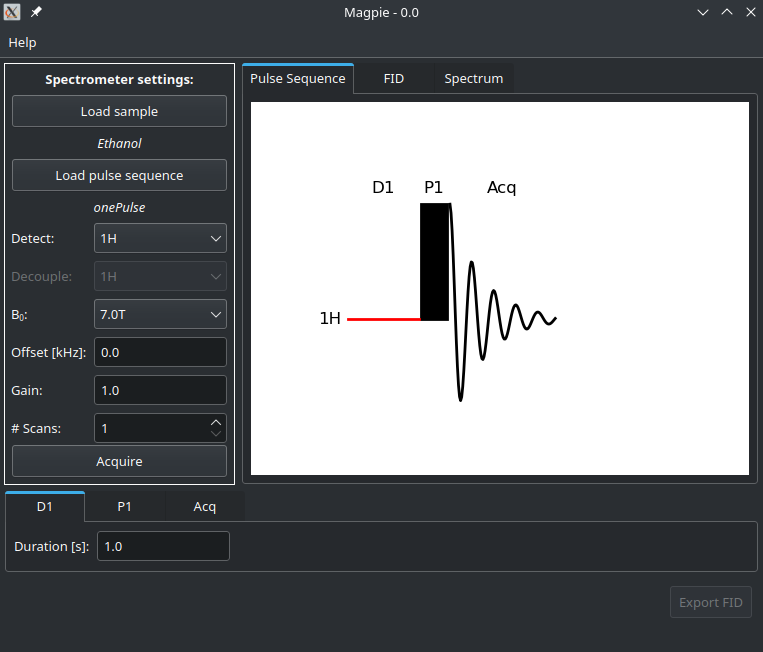
\includegraphics[width=0.7\linewidth]{images/Full_interface.png}
\end{center}
In the sections below, the individual elements are explained.

\subsection{Spectrometer settings}


\begin{center}
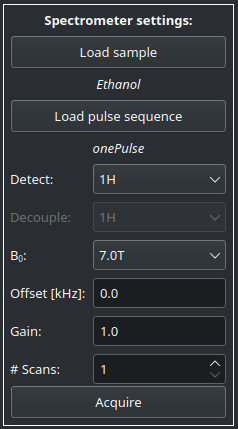
\includegraphics[width=0.3\linewidth]{images/Spec_settings.png}
\end{center}
In the left of the Magpie screen, the spectrometer settings can be put in. These are all settings that are not specific to a pulse sequence. Also, the buttons to load a sample and a pulse sequence are contained here. Below is a list of the settings and their description.

\begin{itemize}
\item \textbf{Load sample:} Opens a file dialog to brows for a sample file. More info can be found in \autoref{sec:sample}. The file should have extension \texttt{.txt}.
\item \textbf{Load pulse sequence:} Opens a file dialog to brows for a pulse sequence file file. More info can be found in \autoref{sec:pulseseq}. The file should have extension \texttt{.csv}.
\item \textbf{Detect:} The nucleus to detect. In principle, any nucleus can be detected. For the moment, we limit the selection to $^1$H and $^{13}$C though. This is a design choice to not overflow the user with obscure nuclei.
\item \textbf{Decouple:} The nucleus that is decoupled during a decoupling pulse sequence element. Only active if the pulse sequence has a decouple element.
\item \textbf{B$_\mathbf{0}$:} The main magnetic field strength in Tesla. Magpie supports any magnetic field strength. For now, we decide on using a dropdown box with only common fields. This is the teach the user that in reality the magnetic field cannot easily be changed to whatever we want.
\item \textbf{Offset [kHz]:} The transmitter offset in kHz. This can be used to fine-tune the center frequency of the experiment. It defines the center of the spectrum, as well as the frequecy on which any pulses are given.
\item \textbf{Gain:} The gain factor of the receiver. All signals are multiplied by this value before detection. Note that, contrary to most real-life spectrometers, Magpie uses a linear scale, and does not work in dB.
\item \textbf{\# Scans:} The number of individual scans that need to be recorded. All scans are automatically summed.
\end{itemize}

\subsection{Pulse sequence settings}\label{sec:seq_settings}

\begin{center}
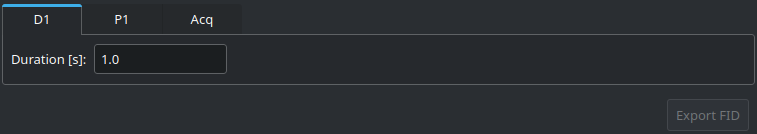
\includegraphics[width=0.9\linewidth]{images/Sequence_settings.png}
\end{center}
In the bottom of the Magpie interface, the pulse sequence settings are defined. Each tab represent a separate element of the pulse sequence. The names of the tabs are equal to the names of the elements, as defined in the pulse sequence file. The pulse sequence diagram (in the plot window) always highlights the element which settings tab is currently showing. More info on pulse sequences, and the relevant settings per element can be found in \autoref{sec:pulseseq}.

\subsection{Plot windows}
The plot window contains three tabs: Pulse sequence, FID, and Spectrum. These are explained below.
\subsubsection{Pulse sequence}\label{sec:inter:pulse}
\begin{center}
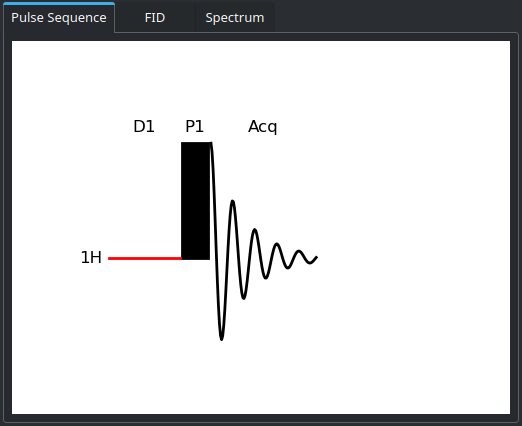
\includegraphics[width=0.9\linewidth]{images/Plot_sequence.png}
\end{center}
The pulse sequence tab displays a diagram of the current pulse sequence. The current element that is selected is displayed in red. Left-clicking on an element changes the selection. The sequence settings tab (see \autoref{sec:seq_settings}) folows this selection (and vice-versa).

The labels displayed above the sequence elements are those as defined in the pulse sequence file. The tabs in the sequence settings window also have this name.

The elements in the pulse sequence each have a unique pictorial representation. The style of the elements is not updated depending on the pulse sequence settings (e.g.\ a pulse with amplitude 0 is not shown as a much lower rectangle).


\subsubsection{FID}\label{sec:FID}
\begin{center}
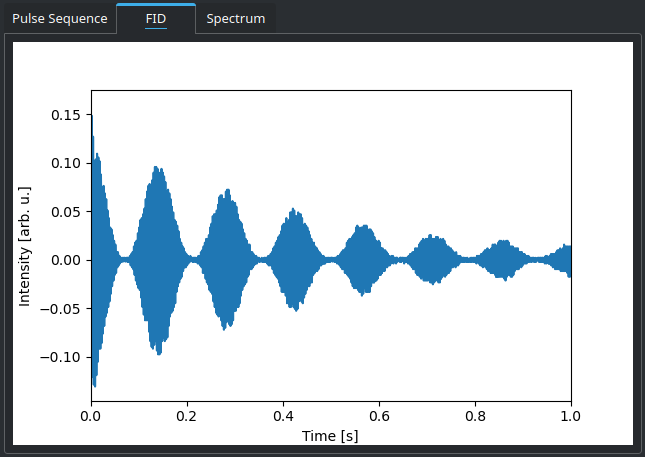
\includegraphics[width=0.9\linewidth]{images/Plot_FID.png}
\end{center}
The FID tab shows the FID (time signal) of the simulated data. If there is no data, no plot is shown. The y-axis has the signal intensity. Although it is in arbitrary units, the maximum value is 1. Any signals high than that will be rounded to 1. For negative intensity the limit is $-1$. These situations relate the `receiver overflow' in real spectrometers, that happens when signals are to strong to properly digitize.

The plot supports the following mouse-based zoom-controls:

\begin{itemize}
\item Dragging a box while holding the left mouse button creates a zoombox, and will zoom to that region.
\item Dragging while holding the right mouse button drags (i.e.\ pans) the spectrum. Doing this while holding the Control button pans only the x-axis, holding Shift pans only the y-axis.
\item Double clicking with the right mouse button resets the view to fit the whole plot (both x and y).
\item Scrolling with the mouse wheel zooms the y-axis. Doing this while also holding the right mouse button zooms the x-axis. By holding Control the zooming will use a larger step size. 
\end{itemize}


\subsubsection{Spectrum}
\begin{center}
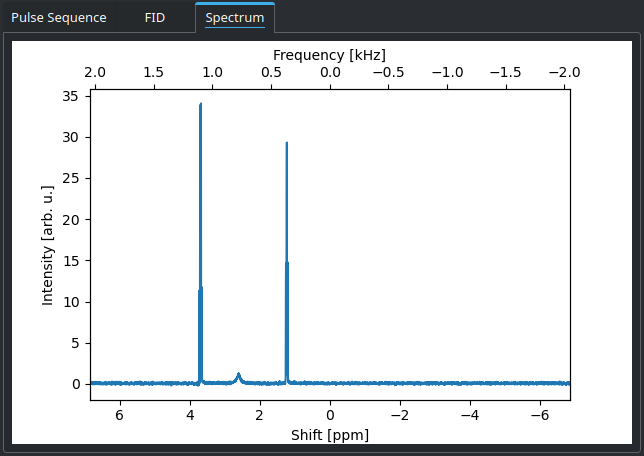
\includegraphics[width=0.9\linewidth]{images/Plot_Spectrum.png}
\end{center}
The Spectrum tab shows the signal after Fourier transformation. Two x-axes are plots:
\begin{itemize}
\item Bottom x-axis: Has the axis in ppm. Here, 0 ppm relates to the signal of the ppm reference for the measured nucleus. If the spectrometer offset is changes, the 0 ppm position can shift in the spectrum.
\item Top x-axis: Has the axis in kHz. For this axis, 0 kHz is always defined in the center of the spectrum. When adjusting the spectrometer offset, this axis can be used to find the desired shift.
\end{itemize}


The spectrum plots has the same zoom controls as the FID plot (see \autoref{sec:FID}).

\section{Sample definition}\label{sec:sample}
Sample files for Magpie need to be in a specific definition. They need to be text files with \texttt{.txt} extension.

The file should start with a header:
\begin{verbatim}
###SAMPLE###
\end{verbatim}
Below this, on optional statement regarding the sample amount (concentration) can be made:

\begin{verbatim}
amount 1 
\end{verbatim}
In this case, the scaling is set to \texttt{1}, so it has no effect.

After this, a molecule can be defined. The sample file can hold multiple molecule definitions. Within this block, the spins are set, as well as the overall relaxation times and the J-couplings.

The statements are:

\begin{center}
\begin{tabular}{lp{5cm}p{6cm}}
\toprule
\textbf{Statement} & \textbf{Input} & \textbf{Description} \\
\midrule
\rowcolor{gray!30!white}
\texttt{amount} & amount & molecule amount\\
\texttt{T1} & T1 & Overall T1, in seconds (optional)\\
\rowcolor{gray!30!white}
\texttt{T2} & T2 & Overall T2, in seconds (optional)\\
\texttt{T2prime} & T2prime & Overall T2prime, in seconds (optional)\\
\rowcolor{gray!30!white}
\texttt{spin} & isotope shift multiplicity & For example: \texttt{1H 1.2 3}\\
\texttt{spin} & isotope shift multiplicity T1 T2 T2prime & Spin definition including relation times. These are used in favour of the overall relaxation times, if set. Values can be set empty by an underscore (\_) \\
\rowcolor{gray!30!white}
\texttt{J} & spin1 spin2 strength & Set J-coupling in Hz between two spin indexes. Number order as the spins are defined. For example: \texttt{J 1 2 9.6}\\
\texttt{Jmatrix} & matrix & Set J-coupling in Hz between all spins in matrix format. Example for two spins: \texttt{[[0,10],[10,0]]}, setting 10 Hz coupling. Size needs to be n\_spins x n\_spins. When used the, regular \texttt{J} statement cannot be used.\\
\rowcolor{gray!30!white}
pair & isotope shift1 shift2 k amp1 amp2 T1\_1 T1\_2 T2\_1 T2\_2 &  Sets a spin-pair with exchange between them. \texttt{amp} sets the multiplicity. Individual T1 and T2 times can be set, or set to empty by an underscore (\_). No J-couplings can be set to these spins.\\
\bottomrule
\end{tabular}
\end{center}

Either \texttt{Jmatrix} or \texttt{J} statements are allowed. Not both.
Spin statements can lack all the relaxation times, or have a \_ instead.
If a relax time not defined for a spin, it needs to use the global molecule relaxation time.
These are also optional, but if they lack, the individual spin lifetimes need to be all there.

An example definition could be the following sample:
\begin{verbatim}
###SAMPLE###
amount 1
###MOLECULE###
amount 0.1
T1 5
T2 0.5
T2prime 10
spin 1H 1.2 3
spin 1H 3.6 2
J 1 2 7
\end{verbatim}
Here we set a two spin system, with shifts 1.2 and 3.6 ppm, multiplicities 3 and 2. There is a 7 Hz J-coupling between the spins. All nuclei have the same relaxation times, set at 5, 0.5 and 10 s for T1, T2 and T2prime respectively. The overall intensity scaling is set at 1, and the molecule itself has scaling 0.1.

A more complicated sample could be ethanol:
\begin{verbatim}
###SAMPLE###
amount 1
###MOLECULE###
amount 0.98 
T1 5
T2 0.5
T2prime 10
spin 1H 1.226 3
spin 1H 3.692 2
spin 1H 2.605 1 _ 0.01 0.1
J 1 2 7
###MOLECULE###
amount 0.01 
T1 5
T2 1
T2prime 10
spin 1H 1.224 3
spin 1H 3.692 2
spin 1H 2.605 1 _ 0.01 0.1
spin 13C 18.1 1 _ _ 7
J 1 2 7
J 1 4 125
###MOLECULE###
amount 0.01 
T1 7
T2 1
T2prime 10
spin 1H 1.226 3
spin 1H 3.692 2
spin 1H 2.605 1 _ 0.01 0.1
spin 13C 57.8 1 _ _ 7
J 1 2 7
J 2 4 125
\end{verbatim}
Here we set three molecules: with no 13C nucleus, and both options with a single 13C nucleus (the 13C-13C variant is too low in intensity to care about). The amount of the molecules is set to follow the natural abundance. For the OH peak (at 2.6 ppm), a separate set of relaxation times is set, as to have a shorter T2 and T2prime, to include the fact that this signal is usually exchanging causing line broadening. J-couplings are ste between the 1H nuclei of the CH$_3$ and CH$_2$ groups, as well as between the 13C nuclei and their directly bonded 1H nuclei. 

\section{Pulse sequence definition}\label{sec:pulseseq}
Magpie reads pulse sequence in comma separated format (\texttt{.csv}). Each sequence element is on its own row. Default settings for its parameters are given in columns with the correct column name. For each sequence element, magpie only looks for the columns needed for that element. Other columns can be left empty, if a specific sequence element does not need those.

Below, the currently supported sequence elements are listed, along with the required columns.

\begin{center}
\begin{tabular}{lp{3.5cm}p{7.5cm}}
\toprule
Element type & Required columns & Description \\
\midrule
\rowcolor{gray!30!white}
\texttt{delay} & \texttt{time} & Set a delay during which nothing is done.\\
\texttt{pulse} & \texttt{time}, \texttt{amp}, \texttt{phase} & Defines a pulse with amplitude in kHz and a phase in degrees. Phase can also be a list (e.g.\ [0,90]) to define a phase cycle.\\
\rowcolor{gray!30!white}
\texttt{FID} & \texttt{time}, \texttt{amp} & Measure the FID, with \texttt{time} the acquisition time in seconds, and \texttt{amp} the amount of points. The receiver phase is always 0, and cannot be phase cycled.\\
\texttt{sat} & & Defines a saturation element. Sets all magnetization to 0. Has no further settings.\\
\rowcolor{gray!30!white}
\texttt{shapedPulse} & \texttt{time}, \texttt{amp}, \texttt{phase}, \texttt{shapeFile} & Defines a pulse with an amplitude shape. Has the same definitons as the \texttt{pulse} element. Additional is the \texttt{shapeFile} column, which should point to a shape file. Can be just a name if the shape file is one of the default shapes. See more in \autoref{sec:shape}.\\
\bottomrule
\end{tabular}
\end{center}

The supplied \texttt{.csv} file should contain several elements as described above. The element type should be supplied, as well as a name of the element. The name is used in the Magpie interface to identify the element in the pulse sequence visualization, as well as in the settings tabs.

An example for a one pulse sequence is given below:

\begin{verbatim}
name,type,time,amp,phase
D1,delay,1
P1,pulse,2.5e-6,100e3,-90
Acq,FID,1,4096
\end{verbatim}
The first column supplies the name of each element, the second the type. Other columns are used to define the starting values of required inputs. The elements defined in this sequence are:
\begin{itemize}
\item A delay with name `D1' and default time of 1 s.
\item A pulse with name `P1' with time 2.5 $\muup$s, amplitude of 100 kHz and pulse phase $-90^\circ$.
\item An FID detection block called `Acq' with time of 1 s, and 4096 points.
\end{itemize}
The resulting sequence is the one displayed in \autoref{sec:inter:pulse}.

An echo sequence can be defined as:

\begin{verbatim}
name,type,time,amp,phase
D1,delay,1,,
P1,pulse,2.5E-06,100000,"[90,270,90,270]"
t1,delay,0.1,,
P2,pulse,5E-06,100000,"[90,0,270,180]"
t2,delay,0.1,,
Acq,FID,1,4096,
\end{verbatim}
Here, we have two pulses and two extra delays. The pulses have a 4 step phase cycle. Note that phase cycles always need to be the same length for all pulse element in the sequence. The phases are defined with respect to the receiver phase, which is always 0, and cannot be phase cycled.


\subsection{Shape files}\label{sec:shape}
Shape files are defined as a text file with a list of float values. Every entry is on a separate row. Each value indicates the relative pulse amplitude at that point. The phase cannot be changed at the moment.

Note that the overall maximum amplitude of the pulse is equal to $\text{amp}_\text{pulse} \cdot \text{amp}_\text{shape}$. It is recommended therefore to set the maximum amplitude in the shape file to $1$, to avoid confusion.

When using the shape, Magpie treats it as a series of pulses. The length of each sub-pulse is set by the total pulse length divided by the number of steps defined in the shape file. Higher resolution pulses can therefore be obtained by supplying a higher resolution shape file. Note that the simulation time will increases by doing this.




\section{Data output}
Magpie is designed to interface with the \texttt{ssNake} program.\footnote{\url{https://www.ru.nl/science/magneticresonance/software/ssnake/}} The default output is a \texttt{.mat} file in the same style as \texttt{ssNake} saves. The button `Export FID' can be used to save the current dataset.



\section{Simulation background}
Magpie uses a classical simulator, so no quantum effects are included. J-couplings are therefore included only as their weak coupling limit, and no coherence between the J-states exists.

Firstly, the sample file is processed, and divided in individual spins. J-coupled states are treated as separate spins, with a different Larmor frequency. For example, a spin which couples to a single $^1$H nucleus with a coupling constant of 10 Hz is subdivided in two spins with +5 and -5 Hz Larmor frequency and half the magnetization.

After this is done, we can define each spin with 6 properties:

\begin{equation}
  S = \left( \begin{array}{c}
M_x \\
M_y \\
M_z \\
M_0 \\
T_1 \\
T_2\\
  \end{array} \right) \quad .
\end{equation}
The spins start with $M_x == M_y == 0$. The total magnetization, due to the amount of spins of a particular site in a molecule, and the amount of the molecule in the sample, is hold in the $M_0$ value, which is also need to calculate the $T_1$ effects.

With the information per spin, the system changes over time can be calculated using the Bloch equations. This is done by using a ODE solver, for each spin individually. Each spin in analysed in a rotating frame rotating at its Larmor frequency, to improve the accuracy and speed of the ODE solver.

The final state after a scan has been calculated becomes the initial state for the next scan. In this way, system history is taken into account, and a proper experiment needs a recovery time of 3-5 times $T_1$ between scans, equalling reality.

For each element in the pulse sequence, the initial state of the spin is taken, and the final a the end of the sequence element is calculated. Only for the \texttt{FID} element, more intermediate values are calculated, in line with the sampling frequency that is specified in the experimental settings.


\subsection{T2prime}
T2prime effects are a collective property relate to the measurement setup of an NMR experiment and the sample being measured. While $T_2$ represent the unrecoverable loss of coherence of a state, T2prim effects describe the loss of coherence due to macroscopic effects. This relates for example to a sample tube in an inhomogeneous magnetic field. Signals will decay faster than the true $T_2$, as the XY-magnetization of spins in different locations in the tube will precess at a different rate. Using a spin echo, for example, the full alignment can be recovered, making it a different process than $T_2$.

Magpie can include T2prime effects in its calculations. It does this by creating a series of duplicate spins, at slightly different Larmor frequency. The sum of all these lines in the spectrum follows a Lorentzian shape, and can be seen as the magnetic field profile over the sample. The width of the envelope is calculated based on the supplied T2prime for each spin. The amount of sub-sampled spins is defined by the T2prime value, and the $T_2$ value of the original spin.

\subsection{Exchange}

\section{Contact}
To contact the \texttt{magpie} team write to \texttt{ssnake@science.ru.nl}.

\bibliographystyle{BibStyle}
\bibliography{ReferenceManual}

\end{document}
